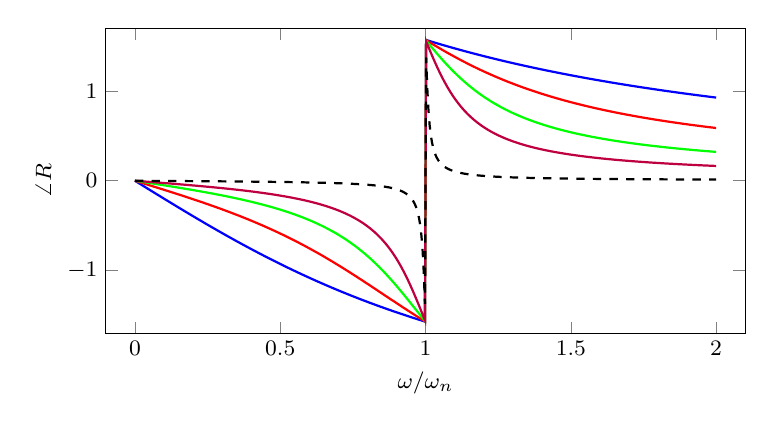
\begin{tikzpicture}[scale=1]
	\footnotesize
	\begin{axis}[
		width=0.8\textwidth,
		height=0.45\textwidth,
		xlabel={$\omega/\omega_n$},
		ylabel = {$\angle R$},
		xmax=2.1,
		xmin=-0.1,
		ymax=1.7,
		ymin=-1.7,  
		samples=500]
		
		
		\def\k{1};
		\def\zetaA{1};
		\def\zetaB{0.5};
		\def\zetaC{0.25};
		\def\zetaD{0.125};		
		\def\zetaE{0.01};		
		
		\addplot[blue, thick, domain=0:2] (x, {rad(atan(-(\zetaA*2*\k*x)/(\k*(1-x^2))))});
		\addplot[red, thick, domain=0:2] (x, {rad(atan(-(\zetaB*2*\k*x)/(\k*(1-x^2))))});
		\addplot[green, thick, domain=0:2] (x, {rad(atan(-(\zetaC*2*\k*x)/(\k*(1-x^2))))});
		\addplot[purple, thick, domain=0:2] (x, {rad(atan(-(\zetaD*2*\k*x)/(\k*(1-x^2))))});
		\addplot[black, dashed, thick, domain=0:2] (x, {rad(atan(-(\zetaE*2*\k*x)/(\k*(1-x^2))))});
		
		% Marks for damped resonance
%		\addplot[green, mark=*, domain=0:2] ({sqrt(1-2*\zetaC^2)}, {1/sqrt(\k^2*(1-(sqrt(1-2*\zetaC^2))^2)^2 + (\zetaC*2*\k*(sqrt(1-2*\zetaC^2)))^2)});
%		\addplot[purple, mark=*, domain=0:2] ({sqrt(1-2*\zetaD^2)}, {1/sqrt(\k^2*(1-(sqrt(1-2*\zetaD^2))^2)^2 + (\zetaD*2*\k*(sqrt(1-2*\zetaD^2)))^2)});
		
%		\draw [thick, dashed] (axis cs: 1, 0) -- (axis cs: 1,5);
%		\node at (axis cs: -0.05, 1) [] {$k$};
		
%		
%		\node at (axis cs: 1.6, 2) [blue,anchor=west] {$\zeta=1$};
%		\node at (axis cs: 1.6, 2.4) [red,anchor=west] {$\zeta=0.5$};
%		\node at (axis cs: 1.6, 2.8) [green,anchor=west] {$\zeta=0.25$};
%		\node at (axis cs: 1.6, 3.2) [purple,anchor=west] {$\zeta=0.125$};
%		\node at (axis cs: 1.6, 3.6) [black,anchor=west] {$\zeta=0$};
		
	\end{axis}
	
\end{tikzpicture}